\chapter{Описание предлагаемого подхода}
\label{chapter2}

\section{Рассматриваемая оптимизационная задача}
\subsection{Задача Needle}
Задача Needle, которую иначе можно назвать "иголка в стоге сена", сформулирована следующим образом: 

Для всех $z \in \{0, 1\}^n \;\;\; $  
    \begin{math} 
    f_{z} : \{0, 1 \}^n \rightarrow \{0,1\}; x \rightarrow  \left\{ \begin{array}{ll}
    1 & \textrm{$x = z$}\\
    0 & \textrm{$x \ne z$}
    \end{array} \right.
    \end{math}

Needle является одной из сложных задач, так как за каждый запрос алгоритм получает лишь знание, совпадает ли запрос с оптимумом или нет, и никаких выводов о других запросах сделать не может. 

Вычислительная сложность Needle по отношению ко всем возможным
алгоритмам равна \frac{2^n + 1}{2}. Это следует из принципа минимакса Yao \cite{5} время работы какого-либо алгоритма не превосходит среднего времени
работы (усредняемого по всем задачам класса) лучшего из детерминированных алгоритмов. Так как за каждый запрос алгоритм получает лишь знание, совпадает ли запрос с оптимумом или нет, то никаких выводов о других запросах он сделать не может, и единственное, что он может сделать - не запрашивать уже запрошенное повторно. Таким образом, лучший детерминированный алгоритм просто делает все возможные запросы по порядку, и среднее число запросов до оптимума - ровно $\frac{2^n + 1}{2}$

Такое же время работы у алгоритма, который генерирует случайную перестановку чисел от 0 до $(2^n - 1)$ и спрашивает их в этом порядке. Верхняя и нижняя оценка совпадают.

Идеи решения задачи Needle могут помочь в будущем в исследовании других задач, в частности, оценить разрешению прохода по плато \cite{6}, 

\subsection{Описание подхода}
Будем рассматривать классы алгоритмов для операторов на несмещенных сложностях. Решения, принимаемые алгоритмом, могут зависеть только от наблюдаемых значений функции, но не от самих точек. Так же алгоритм может делать  запросы, полученные только при помощи несмещенных операторов, обладающих двумя свойствами: инвариантностью относительно перестановки и инвариантностью относительно побитового исключающего или. 
	
Наибольший интерес представляют собой алгоритмы для операторов  несмещенных сложностей арности k = 1, 2, 3.

Время работы black-box алгоритма оценивается числом запросов к черному ящику,  то есть это ожидаемое число запросов до точки  нахождения оптимума.
	
Подсчет верхних оценок сводится к разработке алгоритма и оценке времени его работы.
	
Подсчет нижних оценок сводится к нахождению общего вида всех алгоритмов данного класса, нахождению вещественнозначных параметров, однозначное определяющих работу алгоритма, построению выражения, зависящего от указанных параметров и определяющего математическое ожидание времени работы алгоритма, и  минимизации времени работы.  

\subsection{Black-box оптимизация задачи Needle}

Needle является достаточно простой в обычном случае, но при этом достаточно сложна в black-box модификации.

Задача представляется оптимизирующему алгоритму, представленному в виде черного ящика, к  которому можно задавать запросы, и он возвращает либо 1, если запрос совпал с загаданной строкой, либо 0 в обратном случае. 

\begin{figure}[H]
\caption{}\label{fig3}
    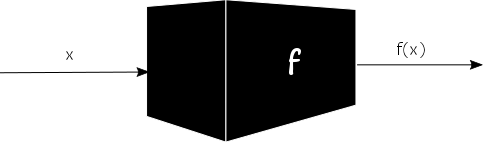
\includegraphics[height=5cm]{ITMO/pic/blackbox.png}
\end{figure}

Запросы к черному ящику можно генерировать либо случайным образом, либо основываясь на результаты предыдущих запросов. В лучшем случае, алгоритм может не запрашивать уже запрошенное повторно.


\chapterconclusion

В данной главе была постановлена решаемая задача, а так же ожидаемые к ней подходы в модели несмещенной blcak-box сложности. Так же были описаны уже существующие решения и оценки их работы, что демонстрирует научную новизну представленной работы. 



